\section{Traffic Engineering}

\subsection{Label Switching}

\paragraph{Packet vs. Circuit Switching}
In packet switching, source sends information as self-contained packets with an address and each packet travels independently to the destination (stateless forwarding at routers) - the destination then recreates the message. In circuit switching, the source first establishes a connection to the destination (reserved bandwidth) and data goes over this reserved path - the connection needs to be established and torn down.

CS guarantees bandwidth and predictable performance, switch design is very simple, adding QoS measures is easy - but, inefficient (esp. for bursty traffic) and overhead.

\paragraph{Virtual Circuits}
Basis of traffic engineering. Forwarding based on a virtual circuit identifier that identify long-lived streams of data that can be scheduled. Each link carries many virtual circuits. Can support various QoS measures (guarantees).

Still does storing and forwarding and still needs buffers. Multiplexing on a link is similar to time sharing (with or without reservations).

\paragraph{Multiprotocol Label Switching (MPLS)}
A layer 2.5 protocol (Ethernet, MPLS header stack, IP) implementing unidirectional virtual circuits = label switched path (LSP) in an IP network. Allows for implementation of TE, QoS, fast reroute, VPNs and more.

A label-switching router inspects an inbound packet's label and input port (per-interface / per-device basis) and according to its forwarding table (single look-up) then decides the output port and next packet label (next hop). At the edge of an MPLS network, labels are either pushed or popped on/off the MPLS label header stack and at the core the top-most label is swapped.

\begin{figure}[h]
	\centering
	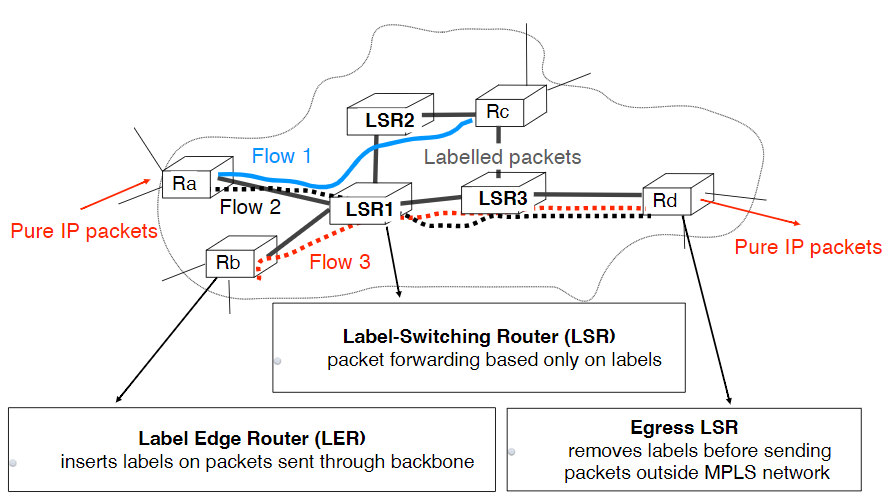
\includegraphics[scale=0.6]{images/1-mpls.PNG}
	\caption{Integrating label swapping and IP.}
	\label{fig:mpls}
\end{figure}

%TODO: more outsourced MPLS info, header etc. also whys
%TODO: lec 4 MPLS in practice (end)?

\paragraph{Forwarding Equivalence Class (FEC)}
Group of IP packets that are forwarded in the same manner. FECs can be used to associate the same label to all packets that belong to the same FEC (usually pushed by a LER). Typically destination IP address, sometimes QoS class.

\paragraph{Distributing Labels}
There are various ways to fill the forwarding tables of all LSRs in a given network. Dedicated protocols, such as LDP and RSVP-TE, can be used to distribute FEC-label mappings. Or mappings can be put inside messages sent by existing routing protocols (that are extensible, such as BGP).

FEC-label mappings are determined by the downstream LSR (destination), which sends them to the upstream one (source). This is either done on demand (space-friendly, not very failure resistant since no backup specified) or in an unsolicited / independent manner (failure resistant by knowing all possibilities, timing is hard).

\paragraph{Label Distribution Protocol (LDP)}
LDP relies on the underlying routing information provided by an IGP (e.g. OSPF, BGP, etc.) in order to forward label packets. Hop-by-hop path through network is determined by the router forwarding information base (FIB, MAC to port mapping). Only signals best-effort (e.g. shortest path) LSPs (no TE - constraints and explicit routes), therefore destination-based forwarding by creating trees with egress LSRs at root.

Neighbor discovery over UDP to figure out if neighboring routers also speak LDP. FEC-exchange over TCP. Egress LSRs map FECs to labels and can also withdraw such mappings (plus other actions).

\textbf{Ordered Label Distribution Control Mode:} Distribution is initiated by egress LSRs by assigning labels to their FECs (all connected IP networks). Other LSR only accept and propagate bindings received by their IGP next-hop if they're part of the shortest path to a destination. Slow but guarantees that the entire LSP is established before labeled packets are forwarded (synchronous).

\textbf{Independent Label Distribution Control Mode:} A downstream LSR binds a label to any FEC it learns in the IGP independently of any other router. For all prefixes a router knows (from an IGP), it will start propagating bindings (asynchronously and independently). Mappings are accepted only of LSR is IGP next-hop (shortest path).

\paragraph{LDP vs. RSVP-TE}
\begin{itemize}
    \item \textbf{Initiate LSP creation:} egress vs. ingress router.
    \item \textbf{Types of signaled LSPs:} unidirectional / multipoint-to-point vs. unidirectional / point-to-point.
    \item \textbf{LSP arbitrary paths:} no, only shortest (IGP-bound) vs. yes.
    \item \textbf{Management:} easy / automatic vs. hard / manual.
    \item \textbf{Scalability:} easy / difficult.
\end{itemize}


\subsection{IP-Based Traffic Engineering}

\paragraph{Bisection Bandwidth}
Cut network in half with half the hosts on one side and half the hosts on the other, take minimum bandwidth of all possible cuts = lower bound on all traffic that can flow through the network.

\paragraph{Router-Level}
Allow a router to use several paths instead of a single one for a given route. Possible with most router implementations.

E.g. ECMP with OSPF. If a router finds several equal cost paths reaching one destination, it may balance its traffic over these paths (independently) = load balancing. Cons: only works for paths with exactly equal cost and each router has to make local decisions.

\textbf{Round-Robin:} Dispatch packets on a per-packet basis on possible paths. Each path carries the same amount of packets. Con: reordering and TCP.

\textbf{Per-TCP Connection:} All packets from the same flow / TCP connection go over the same path. Difficult to find good flow to path mapping without keeping too much state. Use hash functions for that (concatenate IP src, dst, protocol, src and dst port inside bit string and compute hash mod number of paths, slight change in string should produce very different value). Con/challenge: large flows / few flows and polarisation (if all routers use same hash and make the same decisions, avoid by concatenate random value to input string).

\paragraph{Underperforming ECMP}
%TODO paper, lec 4 addendum, collisions cost a lot if you have few flows

\paragraph{Network-Level}
Force aggregate traffic flows to follow some paths inside the network (explicit routes). Possible in some cases by playing with link costs. Challenge: how to optimize those weights s.t. traffic load is balanced = optimisation problem with traffic demands as input (NP-complete). Sub-optimal solution is to search for fitting link weights for each link.

Challenges: traffic matrix can change, limiting frequency of changes to the weights, equipment failure, accepting randomness, etc.

%TODO OSPF weights paper lec 4 addendum end

%TODO examples of opt. problem formulation? objective functions

\paragraph{Advanced Load Balancing}
ECMP has two shortcomings: hash collisions (the less (large) flows, the more costly collisions are) and asymmetry (local decisions without any knowledge of downstream congestion, link failures). We need congestion-aware load balancing decisions.

%TODO papers lec 5 (CONGA, LetFlow)

\paragraph{CONGA}
Handling asymmetry needs non-local knowledge a.k.a. global congestion awareness. To measure congestion, use an extremely fast and low latency distributed protocol that exchanges congestion info in near real-time.

\paragraph{LetFlow}
Congestion-oblivious load balancing scheme that handles asymmetry. Load balancing based on smaller than flows entities (flowlets = (TCP) bursts of the same flow separated by specified amount of time often larger than delay in data center network). Avoids reordering. Flowlet sizes implicitly encode path congestion info (smaller flowlets = congested path since packet drops and backoff mechanism of TCP).

\subsection{MPLS-Based Traffic Engineering}

\paragraph{Resource Reservation Protocol - Traffic Engineering (RSVP-TE)}
Signaling protocol that allows for MPLS-based traffic engineering encapsulated inside IP packets. Edge routers collect traffic statistics and information about link load (to identify congestion). Ingress routers establish LSPs along well chosen paths (not necessarly shortest, paths minimize propagation delay) to divert traffic away from congestion (resources are reserved).

Well chosen paths are found through link attributes (TE metric that specifies cost, max. (available) bandwidth, link class, etc.) propagated by link state routing protocols (e.g. OSPF extension) and applying a fitting algorithm (Dijkstra that minimises one additive constraint, concave constraints by removing all links that don't fit and applying Dijkstra, etc.).

Challenges: when to transmit new link state packets (churn vs. lag, what change is significant, etc.).

\paragraph{Reserving RSVP-TE LSPs}
PATH to request a label (initiated by ingress router) and RESV returns allocated label and reserves requested resources (send by egress router). If a reservation cannot be made, an error message is propagated all the way back to source. Reservation amounts might differ. Requests and responses have to follow the explicit route (ERO) determined by finding a fitting LSP (hop-by-hop path is encapsulated in messages). IP routing does not guarantee symmetric paths. RSVP enables explicit routes (keep state at routers for next hop info). The TE extension introduced the distribution of labels to establish LSPs (otherwise, RSVP just used to reserve resources along an explicit path).

The same pair of source and destination can establish multiple LSPs. Each LSP has an ID.

PATH has strict or loose list of IP addresses (or subnet prefixes / AS numbers) that need to be crossed (loose means more can be added). RESV just goes hop by hop according to router state.

\paragraph{State Maintenance}
Hard-state (circuit-switched networks): state is created at flow establishment and removed at tear down and if an intermediate router crashes, state and reservation are lost. Soft-state (RSVP): each per-flow state has a timer, hosts periodically retransmit PATH and RESV messages, state is automatically reset upon crash, route changes immediately expire old information.

%TODO RSVP intermediate state? details
%TODO RSVP packet format, generally packet formats